% fig_coord_coverage.tex
% TR-35: Full coverage map on (k_ibr, alpha) plane
% Shows all four TR-29 regions plus protection function responsible for each
%
% X-axis: k_ibr [0, 0.22]
% Y-axis: alpha [0, 1.10]
%
% Colours and hatching by primary protection function:
%   k_ibr < 0.06           : dark gray  — no protection possible
%   k_ibr in [0.06, 0.10)  : gray       — 87L only (Region A partial)
%   Region A (k<0.10)      : light gray — 87L (+ 67N for SLG)
%   Region B (k>=0.10, a>0.80): green   — Z2/POTT + 87L
%   Region C               : blue       — Z1 + TDCS + 87L
%   Region D               : teal       — Z1 + 87L
%
% Boundary lines:
%   k_ibr = 0.10 (vertical, I_min_21)
%   k_ibr = 0.06 (vertical, I_min_87L)
%   k_ibr = 0.12 (vertical, C/D boundary)
%   alpha = 0.80 (horizontal, Z1/Z2 boundary)

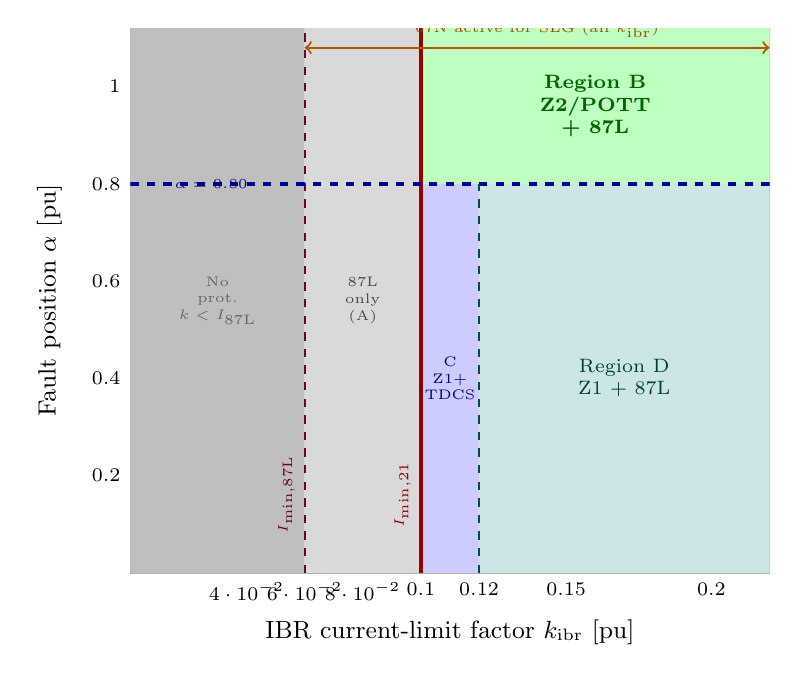
\begin{tikzpicture}
\begin{axis}[
  name        = covax,
  width       = 0.80\textwidth,
  height      = 8.5cm,
  xlabel      = {IBR current-limit factor $k_\mathrm{ibr}$ [pu]},
  ylabel      = {Fault position $\alpha$ [pu]},
  xlabel style= {font=\small},
  ylabel style= {font=\small, yshift=4pt},
  xmin=0.0, xmax=0.22,
  ymin=0.0, ymax=1.12,
  xtick       = {0.04,0.06,0.08,0.10,0.12,0.15,0.20},
  ytick       = {0.20,0.40,0.60,0.80,1.00},
  xticklabel style={font=\scriptsize},
  yticklabel style={font=\scriptsize},
  grid        = major,
  grid style  = {gray!12, dashed},
  tick style  = {draw=none},
  axis line style={gray!60},
]

%% ── No-protection zone: k < 0.06 ────────────────────────────────────────────
\addplot[fill=black!25, draw=none]
  coordinates {(0,0) (0.06,0) (0.06,1.12) (0,1.12)} \closedcycle;

%% ── 87L-only zone: k in [0.06, 0.10) ────────────────────────────────────────
\addplot[fill=gray!30, draw=none]
  coordinates {(0.06,0) (0.10,0) (0.10,1.12) (0.06,1.12)} \closedcycle;

%% ── Region B: k>=0.10, alpha>0.80 — Z2/POTT + 87L ──────────────────────────
\addplot[fill=green!25, draw=none]
  coordinates {(0.10,0.80) (0.22,0.80) (0.22,1.12) (0.10,1.12)} \closedcycle;

%% ── Region C: k in [0.10,0.12), alpha<=0.80 — Z1+TDCS+87L ──────────────────
\addplot[fill=blue!20, draw=none]
  coordinates {(0.10,0) (0.12,0) (0.12,0.80) (0.10,0.80)} \closedcycle;

%% ── Region D: k>=0.12, alpha<=0.80 — Z1+87L ─────────────────────────────────
\addplot[fill=teal!20, draw=none]
  coordinates {(0.12,0) (0.22,0) (0.22,0.80) (0.12,0.80)} \closedcycle;

%% ── Boundary lines ───────────────────────────────────────────────────────────
\addplot[red!60!black, very thick, mark=none]
  coordinates {(0.10,0) (0.10,1.12)};
\addplot[purple!60!black, thick, mark=none, dashed]
  coordinates {(0.06,0) (0.06,1.12)};
\addplot[blue!60!black, very thick, dashed, mark=none]
  coordinates {(0,0.80) (0.22,0.80)};
\addplot[teal!60!black, thick, dashed, mark=none]
  coordinates {(0.12,0) (0.12,0.80)};

%% ── Region labels ────────────────────────────────────────────────────────────
\node[black!60, align=center, font=\tiny]
  at (axis cs:0.03, 0.56) {No\\prot.\\$k<I_\mathrm{87L}$};

\node[gray!60!black, align=center, font=\tiny]
  at (axis cs:0.08, 0.56) {87L\\only\\(A)};

\node[green!40!black, align=center, font=\scriptsize\bfseries]
  at (axis cs:0.16, 0.96)
  {Region B\\Z2/POTT\\+ 87L};

\node[blue!50!black, align=center, font=\tiny]
  at (axis cs:0.11, 0.40) {C\\Z1+\\TDCS};

\node[teal!50!black, align=center, font=\scriptsize]
  at (axis cs:0.17, 0.40) {Region D\\Z1 + 87L};

%% ── SLG annotation (horizontal band, 67N active everywhere) ─────────────────
\draw[orange!70!black, thick, <->]
  (axis cs:0.06, 1.08) -- (axis cs:0.22, 1.08)
  node[midway, above, font=\tiny, orange!60!black]
  {67N active for SLG (all $k_\mathrm{ibr}$)};

%% ── Threshold labels ─────────────────────────────────────────────────────────
\node[purple!60!black, font=\tiny, above=2pt, rotate=90]
  at (axis cs:0.06, 0.15) {$I_\mathrm{min,87L}$};
\node[red!60!black, font=\tiny, above=2pt, rotate=90]
  at (axis cs:0.10, 0.15) {$I_\mathrm{min,21}$};
\node[blue!50!black, font=\tiny, right=2pt]
  at (axis cs:0.01, 0.80) {$\alpha=0.80$};

\end{axis}
\end{tikzpicture}
